%! Licence = CC BY-NC-SA 4.0

%! Author = gianfluetsch
%! Date = 22. Jan 2022
%! Project = icth_summary

\section{Digitale Modulationsarten}

\subsubsection{A}
Die Datensequenz $'1 1 1 0 0 0 0 1 0 1 0 1'$ wird bei einer festen Bitrate von 1 MBit/s mittels vier verschiedener Modulationsarten übertragen. Charakterisieren Sie die verwendeten Verfahren und stellen Sie jeweils die Wertigkeit M der Symbole, d.h. die Anzahl übertragener
Bits pro Symbol fest!
\begin{center}
    \vspace{-8pt}
    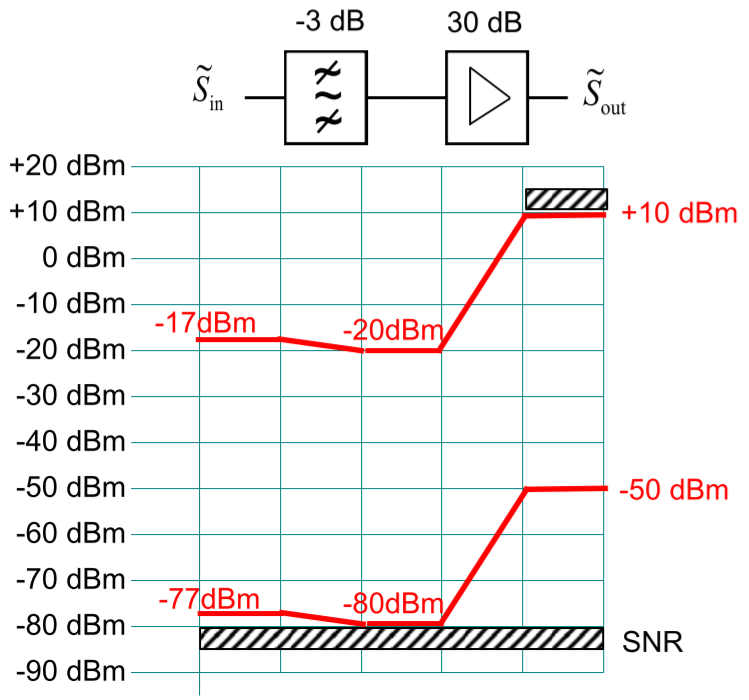
\includegraphics[width=.8\linewidth]{./12-modulationsarten/hs2017}
    \vspace{-8pt}
\end{center}
\begin{center}
    \vspace{-8pt}
    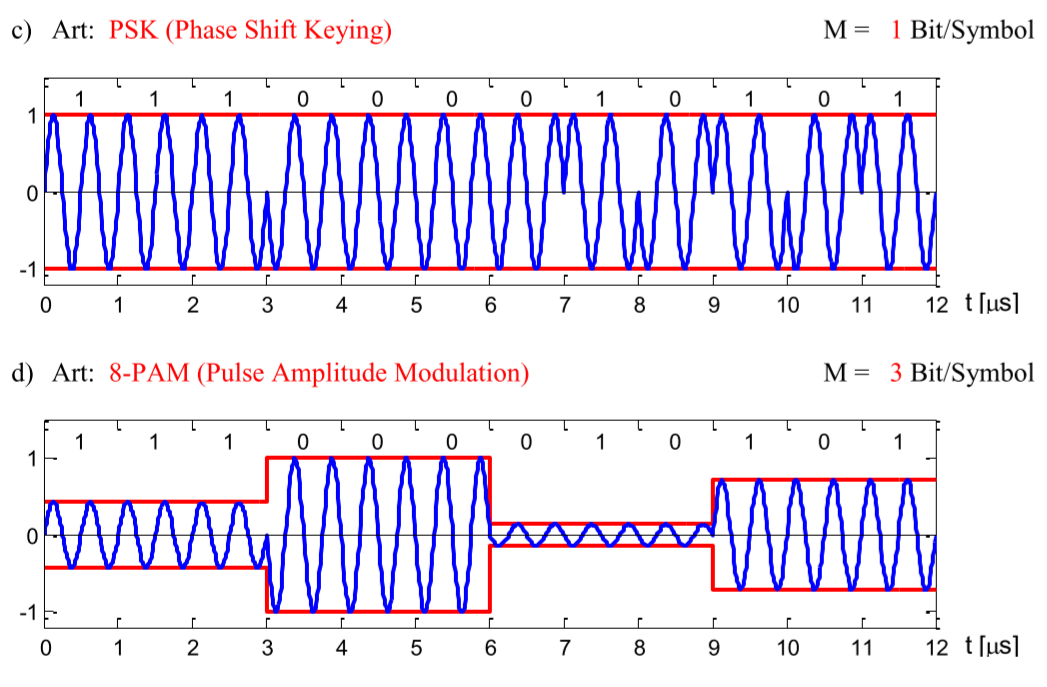
\includegraphics[width=.8\linewidth]{./12-modulationsarten/hs2017_1}
    \vspace{-8pt}
\end{center}

\subsubsection{B}
Bauen sie einen Modulator. Führen Sie dazu die Multiplikation der beiden Signalen $S_N = acos(\omega_Nt)$ und $S_T = bcos(\omega_Tt)$ durch. Betrachten sie das resultierende Signal im Zeit- und Frequenzbereich. Wählen sie für das Modell  die konkreten Grössen $f_T = 3500Hz$ und $fN = 1000...5000Hz$ aus, die Amplituden a und b jeweils 1...10V.\\

\textbf{Interpretieren Sie das Ergebnis mathematisch bezüglich der spektralen Eigenschaften des neuen Signals unter der Annahme, dass $S_N$ ein niederfrequentes Nachrichtensignal und $S_T$ ein hochfrequentes Trägersignal ist.}\\
$S_T*S_N=abcos(\omega_Tt)cos(\omega_Nt)$\\
$=\frac{ab}{2}(cos((\omega_T-\omega_N)t)+cos((\omega_T+\omega_N)t))$\\
Durch die Multiplikation der beiden Signale wird das niederfrequente Signal um die Frequenz des sogenannten Trägersignals (um die Werte $\omega_T -\omega_N$ und $\omega_T+\omega_N$) verschoben oder transponiert. Somit kann das ursprüngliche Signal in einen Frequenzbereich gebracht werden, der sich für eine Abstrahlung eignet (zum Beispiel für eine Radio Amplitudenmodulation in KW, MW oder LW):
\begin{center}
    \vspace{-8pt}
    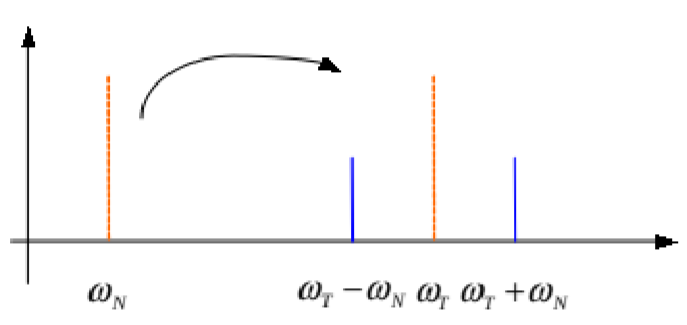
\includegraphics[width=.8\linewidth]{./12-modulationsarten/w11}
    \vspace{-8pt}
\end{center}

Ergänzen Sie einen De-Modulator. Führen Sie dazu wieder die Multiplikation des modulierten Signals mit dem Trägersignal $ST = bcos(\omega_Tt+\varphi )$ durch.
Machen sie beim Demodulationssignal Amplitude, Frequenz und Phase variabel.\\
$S_T*(S_T*S_N)=\frac{ab^2}{2}cos(\omega_Tt)(cos((\omega_T-\omega_N)t)+cos((\omega_T+\omega_N)t))$\\
$=\frac{ab^2}{4}cos((\omega_Tt+\omega_T-\omega_N)t)+cos((\omega_T-\omega_T+\omega_N)t))$\\
$+\frac{ab^2}{4}cos((\omega_Tt+\omega_T+\omega_N)t)+cos((\omega_T-\omega_T-\omega_N)t))$\\
$=\frac{ab^2}{4}cos((2\omega_Tt-\omega_N)t)+cos((2\omega_T+\omega_N)t))$\\
$+\frac{ab^2}{4}(cos(\omega_Nt)+cos(-\omega_Nt))$\\
$=\frac{ab^2}{4}(cos((2\omega_T-\omega_N)t)+cos((2\omega_T+\omega_N)t))+\frac{ab^2}{2}cos(\omega_Nt)$\\

Durch die erneute Multiplikation werden die bereits modulierten Signale nochmals um die Trägerfrequenz $S_T$ verschoben (um die Werte $\omega_T-(\omega_T\pm \omega_N)$ und $\omega_T+(\omega_N\pm  \omega_T)$):
\begin{center}
    \vspace{-8pt}
    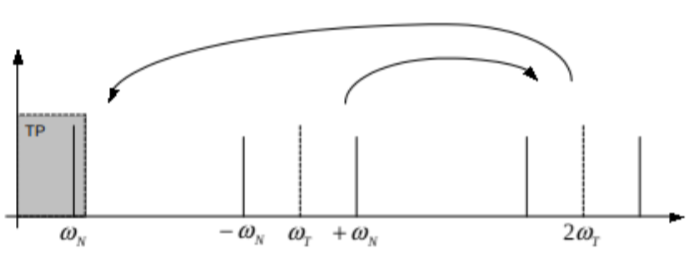
\includegraphics[width=.8\linewidth]{./12-modulationsarten/w11_2}
    \vspace{-8pt}
\end{center}

Mit Berücksichtigung der Phase gilt:\\
$S_T*(S_T*S_N)=\frac{ab^2}{2}cos(\omega_Tt+\varphi )(cos((\omega_T-\omega_N)t)+cos((\omega_T+\omega_N)t))$\\
$=\frac{ab^2}{4}cos((\omega_Tt+\omega_T-\omega_N)t+\varphi )+cos((\omega_T-\omega_T+\omega_N)t+\varphi ))$\\
$+\frac{ab^2}{4}cos((\omega_Tt+\omega_T+\omega_N)t+\varphi )+cos((\omega_T-\omega_T-\omega_N)t+\varphi ))$\\
$=\frac{ab^2}{4}cos((2\omega_T-\omega_N)t+\varphi )+cos((2\omega_T+\omega_N)t+\varphi ))$\\
$+\frac{ab^2}{4}(cos(\varphi +\omega_Nt)+cos(\varphi -\omega_Nt))$\\
$=\frac{ab^2}{4}cos(\varphi )(cos((2\omega_T+\omega_N)t)+\frac{ab^2}{2}cos(\varphi )cos(\omega_Nt)$\\
D.h. ist $\varphi $ ein ungerades Vielfaches von $\frac{\pi}{2}$, so kommt es zur Signalauslöschung.\\

\textbf{Was braucht es, damit die Demodulation fehlerfrei funktioniert?}\\
Damit die Demodulation fehlerfrei funktioniert, braucht es einen Tiefpassfilter, welcher das obere Seitenband der Demodulation herausfiltert. Zudem muss das Demodulationssignal die gleiche Trägerfrequenz und Phasenlage haben.\\

\textbf{Gegeben ist die folgende Prinzipschaltung:}
\begin{center}
    \vspace{-8pt}
    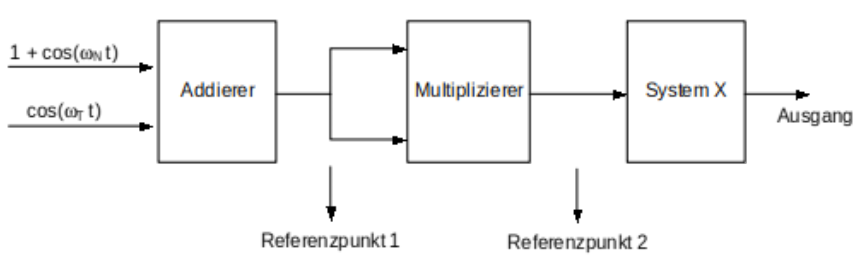
\includegraphics[width=.8\linewidth]{./12-modulationsarten/w11_3}
    \vspace{-8pt}
\end{center}

Hierbei sei $\omega_N$ das Nutzdatensignal und $\omega_T$ das Trägersignal.\\

\textbf{Ermitteln Sie das Frequenzspektrum des Signale mathematisch am Referenzpunkt 1.}\\
$S_1=1+cos(\omega_Nt)+cos(\omega_Tt)$\\

\textbf{Ermitteln Sie das Frequenzspektrum des Signale mit DasyLab und mathematisch am Referenzpunkt 2.}\\
$S_2=S_1^2=(1+cos(\omega_Nt)+cos(\omega_Tt))^2$\\
$=1+cos^2(\omega_Nt)+cos^2(\omega_Tt)+2cos(\omega_Nt)+2cos(\omega_Tt)+2cos(\omega_Nt)cos(\omega_Tt)$\\
$=1+\frac{1}{2}cos(2\omega_Nt)+\frac{1}{2}cos(0)+\frac{1}{2}cos(2\omega_Tt)+\frac{1}{2}cos(0)$\\
$+2cos(\omega_Nt)+2cos(\omega_Tt)+cos((\omega_T+\omega_N)t)+cos((\omega_T-\omega_N)t)$\\
$=2+\frac{1}{2}cos(2\omega_Nt)+\frac{1}{2}cos(2\omega_Tt)$\\
$+2cos(\omega_Nt)+2cos(\omega_Tt)+cos((\omega_T+\omega_N)t)+cos((\omega_T-\omega_N)t)$\\

\textbf{Bestimmen Sie System X so, das am Ausgang ein amplitudenmoduliertes Signal mit Träger anliegt.}\\
Ein Bandpass mit einer unteren Grenzfrequenz von $\omega_T-\omega_N$ und einer oberen Grenzfrequenz von $\omega_T+\omega_N$.